\documentclass[12pt]{article}
\usepackage{hyperref}
\usepackage[utf8]{inputenc}
\usepackage[T1]{fontenc}
\usepackage{graphicx}
\hypersetup{colorlinks=true,linkcolor=blue, linktocpage}
\begin{document}
\section*{R{\o}mmegr{\o}t, 30.12.2018}
\begin{itemize}
\item Oppskrift:
  \begin{itemize}
  \item F{\o}lgte f{\o}lgende
    \href{https://www.matprat.no/oppskrifter/tradisjon/rommegrot/}{oppskrift}
    med 3~dl seterr{\o}mme.  
  \end{itemize}
\item Kommentarer:
  \begin{itemize}
  \item Holdt p{\aa} {\aa} glemme {\aa} glemme saltet.        
  \item Tok ganske lang tid for at sm{\o}r skulle piple ut og
    n{\aa}r det f{\o}rst gjorde det, var det n{\aa}r n{\ae}rmest umulig
    {\aa} fjerne det. Mulig at 1) det var for lite gr{\o}t eller
    2) at jeg ventet for kort tid. Uansett, Gr{\o}ten bar p{\aa}
    ingen m{\aa}te preg av {\aa} ha for mye fett.
  \end{itemize}
\item Konklusjon:
  \begin{itemize}
  \item Smakte ganske godt, i grunnen f{\aa} ting jeg ville endret.
  \end{itemize}
\end{itemize}
\centering
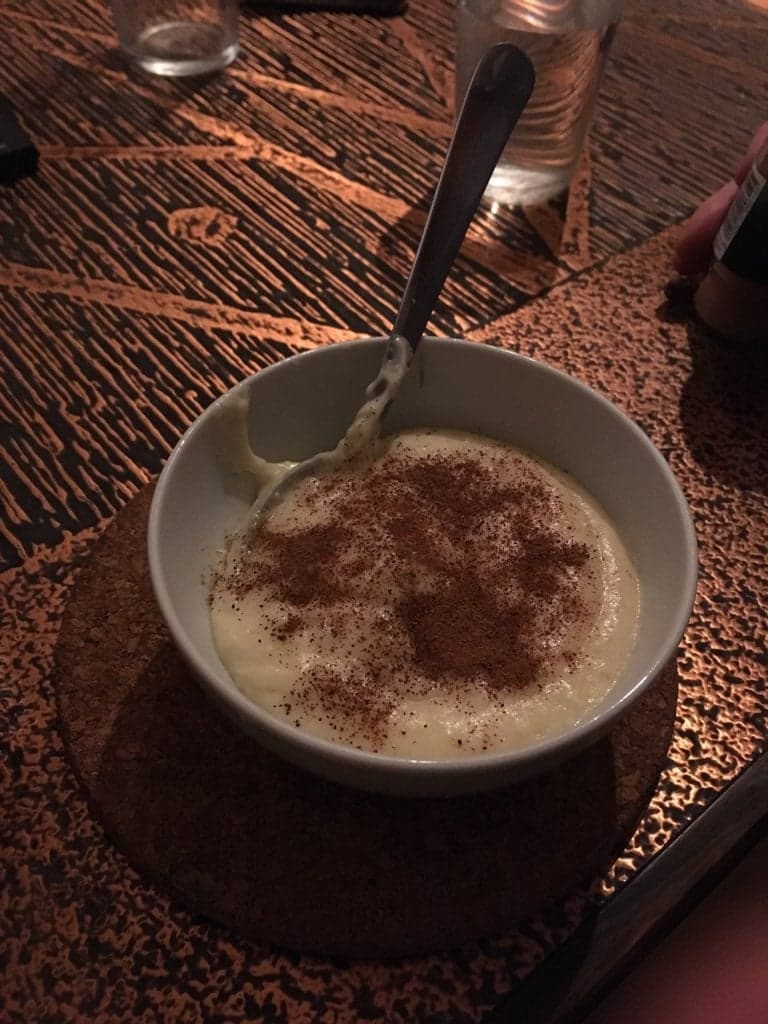
\includegraphics[width=0.33\textwidth]{30-12-2018.jpg}
\end{document}

